\documentclass[11pt]{article}
\renewcommand{\baselinestretch}{1.20} 
\usepackage[utf8]{inputenc}
\usepackage[english]{babel}

\usepackage{graphicx}
\usepackage{wrapfig}
\usepackage{subcaption}
\usepackage{geometry}
\usepackage{xcolor}
\usepackage{float}
\usepackage{mdframed}
\usepackage{booktabs}

\newcommand{\tabitem}{~~\llap{\textbullet}~~}
\geometry{a4paper, total={170mm,237mm}, left=20mm, top=20mm}
\setlength{\abovecaptionskip}{15pt plus 3pt minus 2pt}

\usepackage{fancyhdr}
\usepackage{lastpage}
\pagestyle{fancy}
\fancyhf{}
\rfoot{\thepage}

\begin{document}
    %Title page
    \begin{titlepage}
    \centering
	
\includegraphics[width=0.35\textwidth]{Projectdoc/Assets/Illustrationer/aau_logo_en.pdf}\par\vspace{1cm}
	{\scshape\Large Interaction Design\par}
	\vspace{0.2cm}
	{\huge\bfseries Messages Hidden in Public\par}
	\vspace{0.2cm}
	{\scshape\Large ITC - B125\par}
	\vspace{2cm}
	{\Large\itshape 
    	Mikkel Steen Hansen\\
        Benjamin Bach Jensen\\
        Daniel Vestergaard Jensen\\
    \par}
	\vfill
	\vfill
\end{titlepage}
    
    % Table of contents
    \renewcommand{\baselinestretch}{0.8} 
    \tableofcontents
    \renewcommand{\baselinestretch}{1.20} 
    \newpage
    
    % Short project description
    \section{Short project description}
The goal of the project is to provide people with a tool to maintain some degree of freedom of speech, as well as independent thought, in dictatorial regimes. 
The goal has been chosen due to the potential future risks of ever increasing levels of monitoring across the globe. The intended users are therefore any citizen wanting to discuss the current state of affairs as well as activists that actively try to spread awareness in suppressed populations. The project could also be used by journalists working in the same regions. The military, or indeed intelligence services, might also be able to draw use from the same project. Although the potential benefits are numerous it is important to mention that secure communication could just as well be use by criminals to work against the needs of society.
    
    % Questionnaire description
    \section{Questionnaire methods and execution}
\noindent
This survey [View in appendix \ref{appendix:survey}] intends to explore the level of user awareness regarding privacy. \\
Firstly, it will be determined to which extent the individual user utilizes the internet.\\ 
Secondly, the type of user is determined. \\
Thirdly, the user is asked about their view on their personal privacy on the internet.\\
This is done to explore the possible correlation between amount of use, type of use and privacy view. \\
This information is intended to shed light on whether or not different user groups are likely to use a product capable of enhancing the security of their personal information and freedom on the internet.\\\\
\noindent
The questions in the survey were done in such a way as to allow for classification of the participants.
The survey also asked for permission to conduct follow-up interviews. These interviews intended to provide deeper insight into the reasoning behind certain behaviors. The individuals interviewed would bear close resemblance to one of the personas created to further enhance the insight into these personas.\\\\
\noindent
The intent of the survey was to clarify the archetypes of possible users to allow for the creation of a number of personas. These personas would then be used to create the relevant requirements for the product.
\noindent
Given that the participants have all been present at the university, studying some form of engineering, one possible error is that these participants might have a higher than average technical skill level as well as higher awareness of internet privacy issues.
    
    % Survey findings
    \newpage
    \section{Questionnaire findings}
The group has found, from the 19 responses, that in general about 4 different personas can be found, moreover two further personas exist in different branches. These personas have been separated by whether or not they have actively tried to enhance their own personal security, and their evaluation of how much they feel their privacy is preserved "versus" how much information they think is available about them selves. Some of the participants have filled in their contact information and confirmed their willingness to participate in follow-up interviews.

\subsection{Persona 1 (The non concerned):}
This is the most common persona, with about 8 of the results.
This persona mostly uses their computer for personal matters or entertainment, are active at 7-8 different social media a day,
and uses their home computer for an average of 6 - 8 hours a day.
They are not concerned what others think of them, and therefore also do not hide their personality on social media.
They feel, to a greater extent, than the other personas, that their privacy is preserved on the internet, though they still know that most of their information is publicly available.
They have searched their own name online, mostly for fun, but really do not care about actively trying to enhance their privacy with use of VPN or the like.\\

\textit{From this Persona exists two branches:}
\begin{itemize}
    \item 
    \textbf{The Knowing:}\\
    This branch is highly aware that all of their personal information is publicly available, mainly because of their extensive use of social media.
    \item 
    \textbf{The Ignorant:}\\
    This branch knows that their personal information is public available, though they still believe that some information would be hard, or impossible, to find on the internet.
\end{itemize}

\subsection{Persona 2 (The concerned):}
This is the second most common persona, with about 6 participants fitting the description.
This persona mostly uses their computer for entertainment or work, is active at 6-7 different social media a day,
and uses their devices for an average of 8-10 hours a day.
They are, in some way, concerned what others think of them, and therefore also, to some extend, try to act a certain way on social media, to seem nice and polite.
They feel, to a lesser extend, that their privacy is not preserved on the internet, and here the two branches also differ the most.
They have searched their own name online, and care about trying to enhance their privacy with use of VPN or the like.\\

\textit{From this Persona exists two highly different branches:}
\begin{itemize}
    \item 
    \textbf{The Successful:}\\
    This branch do not feel that their privacy is preserved, and thereby also actively try to enhance their security. They also feel pretty successful in their endeavour, or is rather ignorant of their failure.
    \item 
    \textbf{The Failed:}\\
    This branch do neither feel that their privacy is preserved, despite their high curiosity, nor do they feel that they have succeeded in their security attempts.
\end{itemize}

\subsection{Persona 3 (The user)}
This persona can not really be classified to a single use, as they use their computer for the sake of necessity for school, work or social matters, also they can be active in any average of time and number of social media a day.
They do not act differently on social media or real life as they do not see differentiate between them.
They range all the way from being very concerned about privacy on the internet, to being perfectly happy about it. What they have in common is that no matter their views they have no intention to actively improve upon their privacy.  
They could have tried searching their name, but either way they really do not know to which extent their information is publicly available.

\subsection{Persona 4 (The Extremes)}
This persona either can not fit another perona due to their extremely conflicting responses, perfectly fit a persona but do so to such an extreme degree that it is over the top, or they could have modified their results to a suspicious extent.

    % Requirements
    \newpage
    \section{Requirements}
\textit{To provide secure and yet inconspicuous communication:}
\begin{enumerate}
    \item The system should be able to send messages through some social media.
    \item Messages, sent by the system, should not clearly seem to be a message, in the first place.
    \item The product should not require any personal information itself.
    \item The product should not take longer than 1 minute to install.
    \item 8 out of 10 users should clearly know (after installation) how the product preserves their privacy.
    \item The system should be able to receive and display messages sent by other users.
    \item 9 out of 10 users have to feel that their messages have been securely delivered.
    \item Users have to be able to chain messages together.
\end{enumerate}
\noindent
The first requirement is based on the fact that every persona uses an average of 7-8 different social media a day, thereby a good use for the product could be on any or multiple social media.\\
The second requirement for the product has to be met, as the product otherwise would not enhance the privacy of the individual user.\\
The concerned user [Persona 2] would be highly unwilling to provide any personal information and this leads to the third requirement as they otherwise might not be willing to use the product.\\
\newpage\noindent
The forth requirement regards The user [persona 3] as these would only use the product if it would not require a greater effort.\\
The fifth requirement helps to attract both The concerned and the non concerned [Persona 1 \& 2] as these are both interested in the enhancement of their security but especially the concerned would only use the product if he could see and understand the actual benefit.\\
The sixth requirement is a basic requirement as the product otherwise wouldn't have any use.\\
The seventh requirement is important as the product needs to provide the different users, especially the concerned [Persona 2], with this feeling, as the user otherwise, with particular focus on the normal user [Persona 3], wouldn't use the product more than once.\\
Lastly users like [Persona 2] require the product to function like any other social media, in that they are able to comment and write to each other based on the different posts in relation to one and each other.

\section{Prototype}

\begin{table}[H]
    \begin{minipage}{.5\textwidth}
        \begin{figure}[H]
            \centering
            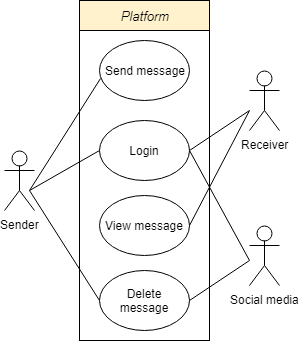
\includegraphics[width=0.75\linewidth]{Projectdoc/Assets/Illustrationer/simple-usecase-eng.png}
            \caption{Usecase diagram}
            \label{fig:usecase}
        \end{figure}
    \end{minipage}
    \begin{minipage}{.5\textwidth}
        \noindent
        Figure \ref{fig:usecase} on the left  describes a conceptual model of what the basic functionality of the inconspicuous communication platform looks like. The model describes how a sender, receiver and a external social media will interface with the system. The "Send message" action will be interfaced with by the sender and will deliver the message to the system for further processing. The "Login" action connects the sender, receiver and social media together. The "View message" action will be interfaced with by the receiver and displays a message from the system. The "Delete message" will be interfaced with by both the sender and the social media and will trigger a message deletion request to the system.
    \end{minipage}
\end{table}

\textbf{Use case \#1, Login.}\\
Object: The user should be prompted for a login, either through a personal social media, or though an anonymous bot.\\
Attributes: Selection of bot, Social media credentials.\\
Operations: Connect the user through the given credentials.\\
Manipulation: Set default settings through sub tap,  Set remember login credentials with checkbox.\\
Next Relationship: Send message[\#2], View message[\#3].\\\\
\newpage
\noindent
\textbf{Use case \#2, Send message.}\\
Object: The user has the option to select a category or thread to submit a new message.\\
Attributes: Selection of post relations, message content.\\
Operations: Post user generated message in relation to the selected thread or category.\\
Manipulation: None.\\
Next Relationship: Login[\#1], Send message[\#2], View message[\#3].\\\\
\noindent
\textbf{Use case \#3, View message.}\\
Object: The user has the option to select a specific message or thread to display.\\
Attributes: Category, Message, Thread.\\
Manipulation: Option to delete a message or thread (If user has ownership).\\
Next Relationship: Login[\#1], Send message[\#2], View message[\#3], Delete message[\#4].\\\\
\noindent
\textbf{Use case \#4, Delete message.}\\
Object: The user have the option to select a specefic message or thread to delete (if user contains ownership).\\
Attributes: Message, Thread, Ownership.\\
Manipulation: Delete a message or thread.\\
Next Relationship: Login[\#1], Send message[\#2], View message[\#3].\\
    
    % Mapping
    \section{Envisioned user experience}
One of the main user focuses, based on the requirements, is the ease of use. The users should not have to learn how to use the communication platform, and therefore it should not defer severely from modern communication platforms. The platform is designed with security in mind, and the design should reflect that. The platforms goal with its content is to deliver meaningful discussion and debates. To promote meaningful content, the posting functionality is built like traditional forums, which puts an emphasis on fewer, but more detailed, posts.  

\section{Prototype documentation}
\subsection{Platform choice}
While modern communication platforms generally have dedicated apps for mobile devices as well as websites for desktop use, it was discussed which of these elements would be most important. If one chose to create an app, it would initially confine the users to their mobile devices. If a web application was built instead, then users might prefer to write forum posts on a computer, but it would be possible to do the exact same on a mobile device through a browser. Therefore, choosing to build an app would limit the usability of the prototype.

\subsection{Prototype choice}
In building the prototype it was discussed whether a lo-fi, mid-fi or a hi-fi prototype would be optimal. On one hand, a lo-fi prototype would be faster to create and would be able to convey the relevant design ideas. On the other hand, a hi-fi prototype would make it possible to interact with it in a way closer to the finished product. If a hi-fi prototype was built now, it would also be possible to reuse the prototype in the final product. Given that our semesterproject requires a GUI, it was deemed sensible to create the front-end in code, without the actual functional back-end. Due to this the prototype could be called mid-fi, as there is no functionality available through the interface, despite the effort put into implementing the interface in HTML and CSS.
\newpage

\subsection{Design choice}
The communication platform is different from modern platforms in a number of ways. The focus on designing an UI that promotes fewer posts and more discussion via replies to the posts. The platform is build with light colors that promote transparency and safety. The overall platform is simple and light with alot of space and without the clutter you will find in other modern platforms. The prototype has three accent colors for its action buttons: the blue color is for navigation and neutral actions, the red is for deletion and backtracking and lastly the green is for sending requests. There are missing symbols and clear indications of the platform's secure features in the prototype, this will be explored later in relevant user studies.

\subsection{Mid-fi prototype}
\begin{table}[H]
    \begin{minipage}{.33\textwidth}
        \begin{figure}[H]
            \centering
            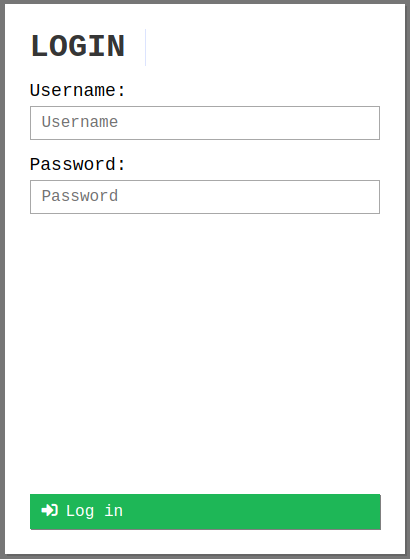
\includegraphics[width=0.95\linewidth]{InteraktionsDesign/Assets/Prototype/1.png}
            \caption{Login screen}
            \label{fig:prototype1}
        \end{figure}
    \end{minipage}
    \begin{minipage}{.33\textwidth}
        \begin{figure}[H]
            \centering
            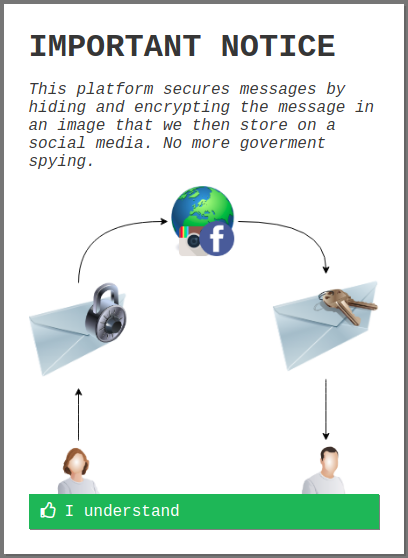
\includegraphics[width=0.95\linewidth]{InteraktionsDesign/Assets/Prototype/2.png}
            \caption{Main menu page}
            \label{fig:prototype2}
        \end{figure}
    \end{minipage}
    \begin{minipage}{.33\textwidth}
        \begin{figure}[H]
            \centering
            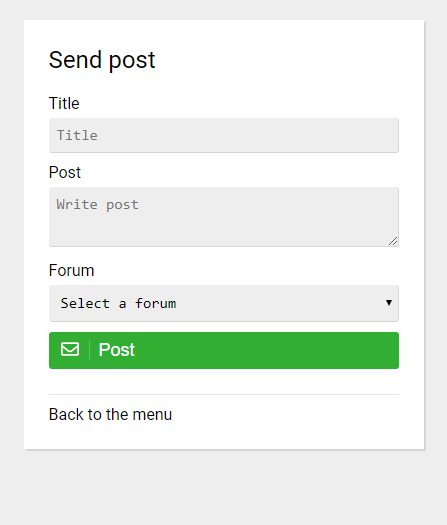
\includegraphics[width=0.95\linewidth]{InteraktionsDesign/Assets/Prototype/3.png}
            \caption{Send forum post}
            \label{fig:prototype3}
        \end{figure}
    \end{minipage}
    \begin{minipage}{.33\textwidth}
        \begin{figure}[H]
            \centering
            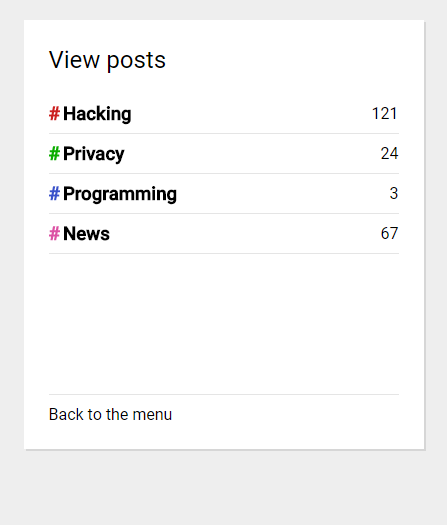
\includegraphics[width=0.95\linewidth]{InteraktionsDesign/Assets/Prototype/4.png}
            \caption{Forum overview}
            \label{fig:prototype4}
        \end{figure}
    \end{minipage}
    \begin{minipage}{.33\textwidth}
        \begin{figure}[H]
            \centering
            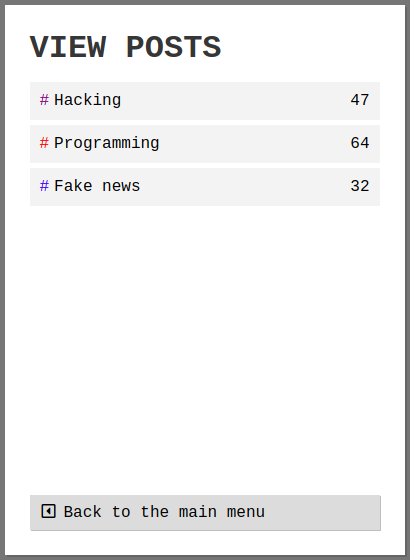
\includegraphics[width=0.95\linewidth]{InteraktionsDesign/Assets/Prototype/5.png}
            \caption{Forum post overview}
            \label{fig:prototype5}
        \end{figure}
    \end{minipage}
    \begin{minipage}{.33\textwidth}
        \begin{figure}[H]
            \centering
            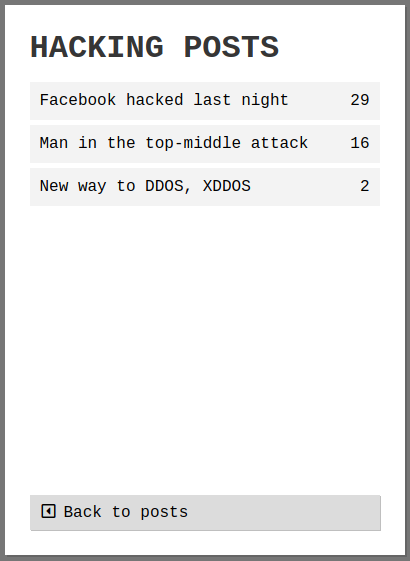
\includegraphics[width=0.95\linewidth]{InteraktionsDesign/Assets/Prototype/6.png}
            \caption{Inside a post}
            \label{fig:prototype6}
        \end{figure}
    \end{minipage}
    \label{fig:prototype}
\end{table}
\newpage
\subsection{Prototype description}
The 6 images above show the most important pages in the application. It starts with the login screen [figure \ref{fig:prototype1}], where the user is prompted with the option to log into the system. In this figure the option to connect to a bot is left out [view usecase \ref{usecase_bot}]. The user is then greeted with a simple menu page, with the option to "Send post", "View posts" and "Logout" [figure \ref{fig:prototype2}]. If "Send post" is selected in the main menu, then a page with three inputs will appear [figure \ref{fig:prototype3}]. These input asks for the post title, message and the desired forum. If you go back to the main menu [figure \ref{fig:prototype2}] and select the "View posts" button, then you will be greeted by a forum overview [figure \ref{fig:prototype4}]. The forum overview displays all the available forum topics, all displayed in different colors. This overview only shows the bare minimum: forum name, color and number of posts inside the forum. If you navigate into a forum, you will get another overview page, this time over forum posts [figure \ref{fig:prototype5}]. The listings on this page displays a snippet of a forum post, with post name, content preview and the number of post replies. If you then go into a forum post, you will get the post content [figure \ref{fig:prototype6}]. This page contains the post content and title, and the option to add or view replies to the post in question.
    
    % User Evaluation
    \section{User Evaluation}
\subsection{Description}

\subsubsection{Introduction and hypotheses}
The user interface has been designed to look similar to current forum-style "social media". This choice of design was made such that the average user would be facing as little a hurdle as possible, in transitioning from their current forum of choice to this product. To test if this is actually the case the following \textit{null hypothesis} is posed:\newline
\textit{ - When presented with a product with similar features, but better security, users will not leave their current daily driver}

\subsubsection{Subjects}
The test subjects in the experiment were found at the university, in or close to our own hall. This means that the subjects in the test were all of rather similar educational programs. This would tend to cause the test subjects to be somewhat similar to our selves in mindset. The test subjects are also probably of a higher than average technical skill level and might be more familiar with forums than the average user.

\subsubsection{Materials}
The prototype is run as a simple interactive website controlled from a browser on a computer. The users use the computer's keyboard and mouse to navigate the prototype. As the prototype is programmed only using HTML, CSS and JavaScript there is no need for extra software other than the web browser.

\subsubsection{Methods and procedure}
\label{procedure}
The experiment is run in two stages: The first stage is using the qualitative method "think aloud", where the user is asked some questions while navigating the prototype. These questions are asked on the fly. The second stage is using the quantitative method "System Usability Scale (SUS)", which is an acknowledged questionnaire, that measures how the usability of the system was. Through these two methods the results can be triangulated to provide more certainty in the experiment.

\begin{figure}[H]
    \centering
    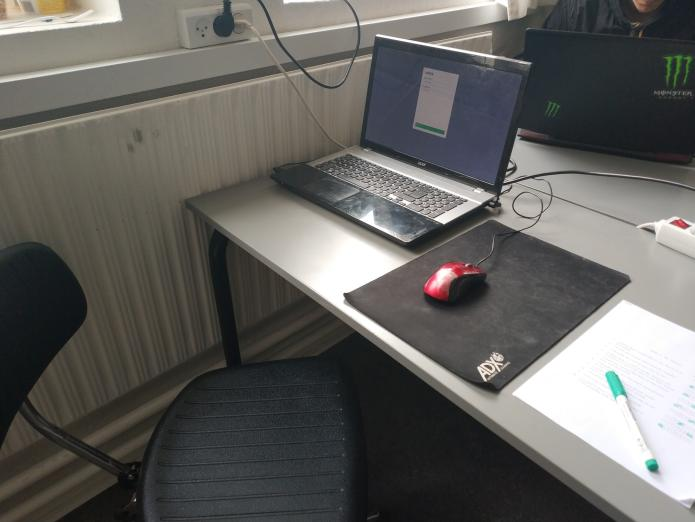
\includegraphics[width=0.75\linewidth]{InteraktionsDesign/Assets/Illustrationer/opstilling.jpg}
    \caption{The prototype is evaluated using this laptop setup, with the browser window in full screen}
    \label{fig:protypesetup}
\end{figure}

\begin{mdframed}[linewidth=0pt,backgroundcolor=lightgray!20,innertopmargin = 0.5cm,innerbottommargin = 0.5cm]
    \begin{enumerate}
        \item Firstly, the subjects are given a small introduction to the prototype. The subject also signs a form informing the subject of the intended use of the data, and their right to stop the evaluation at any time. The subject is sitting on a chair and using the setup seen in figure \ref{fig:protypesetup}.
        \item The subject now take a look on the log-in page of the prototype, and is then asked what they are looking at.
        \item The subject is now provided with the user name "test" and the password "123123", and is asked to log in.
        \item The subject is now asked to navigate the prototype, and find two endpoints:
        \begin{enumerate}
            \item The first navigation task is to send post a post to the forum called "Hacking" [Accessed via figure \ref{fig:prototype4}].
            \item The second navigation task is to find the post named "Facebook hacked last night!", and post a reply [Accessed via figure \ref{fig:prototype7}].
        \end{enumerate}
        \item After the subject has completed the navigation tasks, then he/she is asked about the general impression of the prototype.
        \item Lastly for the "think aloud" test, three additional questions are asked:
        \begin{enumerate}
            \item How clearly was the message of this being a secure platform conveyed?
            \item How could it be more clear?
            \item What will make you change to a more secure messaging platform? (From the main one the subject is using).
        \end{enumerate}
        \item The subject is now handed the SUS questionnaire.
        \item The evaluation ends after asking the subject about how he/she felt the evaluation was handled.
    \end{enumerate}
\end{mdframed}

\subsubsection{Problems}
During the think aloud test it was found that if we answered too many small questions the test could turn into a conversation. Therefore, ones experiment must have a well defined rule set such that the people running the experiment do not disturb the test themselves.\newline
Regarding the SUS some test subjects were confused as to whether they had to answer the survey based on the prototype presented to them or if they had to imagine how the "finished" product would rate on the different scales. This issue made it evident that the individual parts of the experiment need to be thoroughly explained, even when it seems straightforward.

\subsection{Results}
The user evaluation test was executed with a small sample size of 8 participants, they where also subject to the same procedure as described in section \ref{procedure}.

\subsubsection{Think aloud test results}
Common observations from the think aloud test. The full raw data is available in appendix \ref{appendix:thinkaloud}.
\begin{enumerate}
    \item Some participants felt the splash screen did not sufficiently explain the security concept. This refers to both the technical details but also the concept itself. 
    \item At least one participant thought the use of clip art on the splash screen lacked seriousness.
    \item One participant specifically noted, that a graphical explanation of the concept was nice, in contrast to a lot of text.
    \item Every participant thought one thing or another was somewhat unclear or misleading.
    \item Most of the participants thought the prototype was simple in design without much clutter.
    \item Several participants noticed the lack of a "forgot password" option and a "create account" option
    \item No participants were able to guess, that the product could utilise their own social media as part of the security concept.
    \item Some participants noticed that the log-in page gave no hints as to which product they were about to log in to. 
\end{enumerate}

\subsubsection{SUS test results}
Full raw data from the SUS test, can be found in appendix \ref{appendix:susvalues}. The data is also represented in a histogram as shown in Figure \ref{fig:histogram}. The histogram was made with a bin size of 5 and the data has a mean of 79.4 and a standard deviation of 4.49.

\begin{figure}[H]
    \centering
    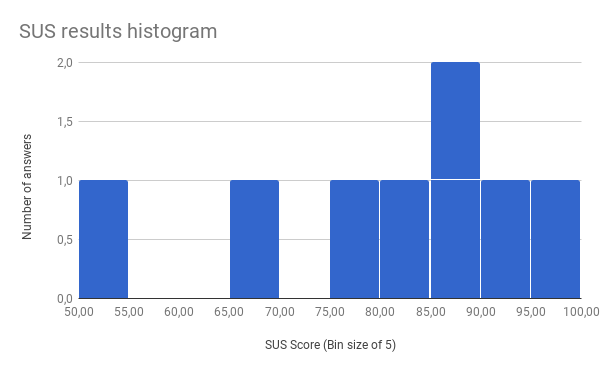
\includegraphics[width=0.75\linewidth]{InteraktionsDesign/Assets/Resultater/histogram_new.png}
    \caption{SUS test results visualised in a histogram with values:
        \mu  = 79.4  \newline SD = 4.49}
    \label{fig:histogram}
\end{figure}

\subsection{Discussion}
If we were to consider the SUS results as a standalone usability measurement, with a score of 68 being the threshold for good usability, then six out of eight test subjects deemed the usability good. However, since the SUS cannot be considered independently and the sample size is quite small, the overall usability might be somewhat lower. This is due to the fact that most of the test subjects thought some elements were lacking in explanation or downright confusing. One participant in particular was surprised that "Send post" referred to making a post on a forum. The participant thought that "Send post" was referring to sending a message to someone in particular. Steps should be taken to prevent such confusion. 
\newline
Another issue that surfaced during the experiment was the subject's understanding of the system's security concept. The splash screen presentation of the concept resulted in a number of problems. First off, at least one participant clicked right past the screen. This allowed for no information to be passed on to the user. Another user found the graphical representation of the concept to be childish, preferring text instead. However, another participant thought that the graphical representation of the concept was really good because this person would not have wanted to read a wall of text. From this it is clear that both types of users exist and they prefer differing communication styles. One might envision a splash screen that asks the user to chose a type of explanation. This is further supported be the fact that two test subjects had the opposite problems. One of these did not understand the splash screen because the subject could not decide how to interpret the images presented and therefore had difficulty understanding the concept. The other user was convinced that the images were to be interpreted in a very particular way. However, this subject then immediately started questioning the validity of the method, despite actual technical explanation being nowhere to be found. Obviously both users would benefit greatly from a longer written explanation. Again one might need to implement two different explanations, one in great technical detail and one in conceptual details. 
Expanding on this the seventh qualitative result further cements that the concept was too poorly explained. Given the fact that the product's most important feature is a specific kind of security that should provide an extensive anonymization capability, it is a must that this is conveyed properly. Furthermore, the understanding of this concept would also be important in using the finalised product since that version would include the option to use anonymous social media accounts as well as one's private account.
    
    % Conclusion
    \section{Conclusion}
From the experiment it has been made evident, that a number of improvements can be made to the prototype. The most important of these is the ability to better explain the security concept, as well as alleviating the confusion caused by small UI elements, which most of the test users experienced.
\noindent
Specifically concerning the null hypothesis posed for the experiment three differing stances seemed to occur. Firstly, some test users said they would be willing to switch to a different product if the other product had the same features, with some features being more important than others though. Secondly, some test users said they would only really consider switching if they had felt severely compromised on their current platform. Thirdly, some users said that a really important thing would be that ones contacts would also switch. Of course some participants could appreciate more than one of these stances.
\noindent
While it was not possible to determine the statistical significance, due to a much too small sample size, it was made clear that a security increase alone might not convince quite as many people to switch to a different platform as one might have otherwise assumed. 
    
    \newpage
    % Appendix
    \section{Appendix}

\subsection{Questionnaire survey}
\label{appendix:survey}
\begin{mdframed}[linewidth=0pt,backgroundcolor=lightgray!20,innertopmargin = 0.1cm,innerbottommargin = 0.5cm]
    \noindent
    \textit{I hereby accept that my answers in this survey can be used in this study, on the condition that my anonymity is guaranteed.}\\
    \begin{tabular}{ll}
        Signature:\qquad
        \begin{left}
            \rule{0.6\textwidth}{.4pt}
        \end{left}
    \end{tabular}
    \begin{enumerate}
        \item What is your age ? \rule{0.1\textwidth}{.4pt}
        \item What are you currently studying ?
        \begin{left}
            \rule{0.46\textwidth}{.4pt}
        \end{left}
        
        \item ~For how long do you use your devices at home on average per day ? (Select \textbf{1})\\
        \begin{tabular}{ll}
            \tabitem Less than 2 hours & [\quad] \\
            \tabitem Around 2 to 4 hours & [\quad] \\
            \tabitem Around 4 to 6 hours & [\quad] \\
            \tabitem Around 6 to 8 hours & [\quad] \\
            \tabitem Around 8 to 10 hours & [\quad] \\
            \tabitem More than 10 hours & [\quad] \\
        \end{tabular}
        
        \item ~What do you primarily use your devices for ? (Select \textbf{at most 3}) \\
            \begin{minipage}{.5\textwidth}
                \begin{tabular}{ll}
                    \tabitem Homebanking & [\quad] \\
                    \tabitem Work & [\quad] \\
                    \tabitem School & [\quad] \\
                    \tabitem Entertainment (Youtube etc.) & [\quad] \\
                \end{tabular}
            \end{minipage}
            \begin{minipage}{.5\textwidth}
                \begin{tabular}{ll}
                    \tabitem Gaming & [\quad] \\
                    \tabitem Social networking & [\quad] \\
                    \tabitem Shopping & [\quad] \\
                    \tabitem Hobby & [\quad] \\
                \end{tabular}
            \end{minipage}
            \\\\
            \begin{tabular}{ll}
                \tabitem Others [Please Write:] &
                \begin{left}
                    \rule{0.35\textwidth}{.4pt}
                \end{left}
            \end{tabular}
        \item ~Which social media / forums do you use ? (Check any that apply) \\
        \begin{minipage}{0.33\textwidth}
            \begin{tabular}{lll}
                \tabitem Facebook & [\quad] \\
                \tabitem Instagram & [\quad] \\
                \tabitem Twitter & [\quad] \\
                \tabitem Reddit & [\quad] \\
            \end{tabular}
        \end{minipage}
        \begin{minipage}{0.33\textwidth}
            \begin{tabular}{lll}
                \tabitem Snapchat & [\quad] \\
                \tabitem Tumblr & [\quad] \\
                \tabitem LinkedIn & [\quad] \\
                \tabitem Steam & [\quad] \\
            \end{tabular}
        \end{minipage}
        \begin{minipage}{0.33\textwidth}
            \begin{tabular}{lll}
                \tabitem Discord & [\quad] \\
                \tabitem Youtube & [\quad] \\
                \tabitem Skype & [\quad] \\
                \tabitem Twitch & [\quad] \\
            \end{tabular}
        \end{minipage}
        \\\\
        \begin{tabular}{ll}
            \tabitem  Others (Please Write) &
            \begin{left}
                \rule{0.52\textwidth}{.4pt}
            \end{left}
        \end{tabular}
        \item Do you feel that you have to act a certain way on social media, \\
        that differs from your normal behaviors ?
        \begin{tabular}{ll}
            No [\quad] & Yes [\quad]
        \end{tabular}
        
        \item If Yes, Why ? and how does it change based on the used platform ? \\
        \begin{left}
            \rule{0.82\textwidth}{.4pt}
        \end{left}\\
        \begin{left}
            \rule{0.82\textwidth}{.4pt}
        \end{left}\\
        \begin{left}
            \rule{0.82\textwidth}{.4pt}
        \end{left}
        
        \newpage
        \item How much do you feel that your privacy is preserved on the internet?:
        
        Not at all [\quad] / Not much [\quad] / To some extend [\quad] / Quiet well [\quad] / It's preserved [\quad]
        
        \item Have you ever searched your own name on Google or other search engines?:
        
        \begin{tabular}{ll}
           Never & [\quad]
        \end{tabular}
        \begin{tabular}{ll}
           Once & [\quad]
        \end{tabular}
        \begin{tabular}{ll}
           Multiple times & [\quad]
        \end{tabular}
        
        \item Do you try to enhance your privacy, on the internet ?
        \begin{tabular}{ll}
            No [\quad] & Yes [\quad]
        \end{tabular}

        If yes, how ? e.g. VPNs, Tor, cookie cleaners... (Please write) \\
        \begin{left}
            \rule{0.5\textwidth}{.4pt}
        \end{left}\\
        If no, why not? (Please write) \\
        \begin{left}
            \rule{0.8\textwidth}{.4pt}
        \end{left}\\
        \begin{left}
            \rule{0.5\textwidth}{.4pt}
        \end{left}
        
        \item ~What information is \textbf{publicly} available about you on social networks? \\
        \begin{minipage}{.5\textwidth}
            \begin{tabular}{ll}
                \tabitem Full name & [\quad] \\
                \tabitem Phone number & [\quad] \\
                \tabitem Age & [\quad] \\
                \tabitem Full address & [\quad] \\
                \tabitem Main mail-address & [\quad] \\
                \tabitem Secondary mail-address & [\quad] \\
                \tabitem Gender & [\quad] \\
            \end{tabular}
        \end{minipage}
        \begin{minipage}{.5\textwidth}
            \begin{tabular}{ll}
                \tabitem Education & [\quad] \\
                \tabitem Occupation & [\quad] \\
                \tabitem Personal images & [\quad] \\
                \tabitem GPS location & [\quad] \\
                \tabitem Interests & [\quad] \\
                \tabitem Civil status & [\quad] \\
                \tabitem Family members & [\quad] \\
            \end{tabular}
        \end{minipage}
        \begin{tabular}{ll}
            \\
            \tabitem  Others (Please Write) &
            \begin{left}
                \rule{0.52\textwidth}{.4pt}
            \end{left}
        \end{tabular}
        \\
    \end{enumerate}
    \\
    \toprule
    \newline\noindent\\
    Filling out the following contacts form confirms that you are willing to, if relevant, further participate in a personal interview:\\\\
    \begin{tabular}{ll}
        \quad E-mail: &
        \begin{left}
            \rule{0.46\textwidth}{.4pt}
        \end{left}\\\\
        \quad Phone number: &
        \begin{left}
        \rule{0.46\textwidth}{.4pt}
        \end{left}
    \end{tabular}
\end{mdframed}

\subsection{Raw data questionnaire}
\label{appendix:rawdata}

\subsubsection{Explanation of certain values}

\noindent\textbf{Category} \hfill \\
Category given based on general observations in the data.
\begin{itemize}
    \item[nck] Persona 1: The non-concerned (Knowing) [Page: \ref{persona11}]
    \item[nci] Persona 1: The non-concerned (Ignorant) [Page: \ref{persona12}]
    \item[con s] Persona 2: The concerned (Success) [Page: \ref{persona21}]
    \item[con f] Persona 2: The concerned (Failed) [Page: \ref{persona22}]
    \item[use] Persona 3: The user [Page: \ref{persona3}]
    \item[ex] Persona 4: The Extremes [Page: \ref{persona4}]
\end{itemize}

\noindent\textbf{Field of study} \hfill \\
Original: What are you currently studying?
\begin{itemize}
    \item[SW] Software students
    \item[ITC] Internet technologies and computersystems students
\end{itemize}

\noindent\textbf{Time on web} \hfill \\
Original: For how long do you use your devices at home on average per day ?  
\begin{itemize}
    \item[1] Less than 2 hours
    \item[2] Around 2 to 4 hours
    \item[3] Around 4 to 6 hours
    \item[4] Around 6 to 8 hours
    \item[5] Around 8 to 10 hours
    \item[6] More than 10 hours
\end{itemize}

\noindent\textbf{Times self searched?} \hfill \\
Original: Have you ever searched your own name on Google or other search engines?
\begin{itemize}
    \item[1] Never
    \item[2] Once
    \item[3] Multiple times
\end{itemize}

\subsubsection{Questionnaire data}
\begin{table}
    \centering
    \begin{tabular}{llllllllll}
    \textbf{Category} & ex  & ex    & nci   & nci   & nci     & nci   & nck  & nck & nck \\
    \textbf{Age} & 25  & 21    & 20    & 20    & 21      & 21    & 23   & 21  & 22  \\
    \textbf{Field of study} & SW  & SW  & SW    & ITC   & SW  & SW    & SW   & SW  & ITC \\
    \textbf{Time on web} & 6   & 5     & 3     & 3     & 3       & 5     & 6    & 6   & 5   \\
    \textbf{Primary internet use:}
    homebank        &     &       & x     &       &         &       &      & x   &     \\
    work            & x   &       &       &       &         & x     &      &     &     \\
    school          & x   &       &       &       & x       & x     &      &     &     \\
    entertainment   &     & x     & x     & x     & x       & x     &      & x   & x   \\
    game            & x   & x     & x     & x     & x       &       &      & x   & x   \\
    social          &     &       &       & x     &         &       &      &     & x   \\
    shop            &     &       &       &       &         &       &      &     &     \\
    hobby           &     & x     &       &       &         &       &      &     &     \\
    \textbf{Change online behavior?} & yes & no    & no    & no    & no      & no    & yes  & no  & no  \\
    \textbf{How preserved? [1 - 5]} & 1   & 2     & 4     & 3     & 3       & 3     & 3    & 5   & 3   \\
    \textbf{Times self searched?} & 3   & 3     & 2     & 1     & 3       & 2     & 3    & 3   & 3   \\
    \textbf{Try to enhance security?}         & yes & yes   & no    & no    & no      & yes   & no   & no  & no  \\
    \textbf{Social media profiles:} &  &  &  &  &  &  &  &  & \\
    Facebook        & x   & x     & x     & x     & x       & x     & x    &     & x   \\
    Instra          &     & x     &       & x     &         &       &      &     & x   \\
    Twitter         & x   &       &       &       &         & x     &      & x   &     \\
    Reddit          & x   & x     & x     &       &         & x     &      &     & x   \\
    Snapchat        &     &       & x     & x     &         &       & x    &     & x   \\
    Tumblr          &     &       & x     &       &         &       &      &     &     \\
    Linkedin        &     &       & x     & x     &         &       & x    &     &     \\
    Steam           & x   & x     & x     & x     & x       & x     & x    & x   & x   \\
    Discord         & x   & x     & x     & x     & x       & x     & x    & x   & x   \\
    Youtube         & x   & x     & x     & x     & x       & x     & x    &     & x   \\
    Skype           &     &       &       &       &         &       & x    & x   &     \\
    Twitch          & x   & x     &       &       & x       & x     &      & x   & x   \\
    \textbf{Public available data:} &  &  &  &  &  &  &  &  & \\
    Full name       &     & x     & x     & x     & x       & x     & x    & x   & x   \\
    Phone           &     & x     & x     &       &         &       & x    & x   & x   \\
    Age             &     & x     &       &       &         & x     & x    & x   & x   \\
    Address         &     & x     &       &       &         &       & x    & x   & x   \\
    Main mail       &     &       & x     &       &         &       & x    & x   & x   \\
    Second mail     &     & x     &       &       &         &       & x    & x   & x   \\
    Gender          & x   & x     & x     & x     & x       & x     & x    & x   & x   \\
    Education       &     & x     & x     & x     &         & x     & x    & x   & x   \\
    Occupation      &     & x     &       & x     &         & x     & x    & x   & x   \\
    Images          & x   & x     & x     & x     &         & x     &      & x   & x   \\
    GPS             &     &       &       &       &         &       &      &     &     \\
    Interests       &     & x     &       & x     &         & x     & x    & x   & x   \\
    Civil           &     & x     &       &       &         & x     & x    & x   &     \\
    Family members  &     & x     &       &       &         &       & x    & x   &     \\
    \end{tabular}
\end{table}
\begin{table}
    \centering
    \begin{tabular}{llllllllll}
    \textbf{Category} & nck & con s & con s & con s & con s/f & con f & conf & use & use \\
    \textbf{Age} & 20  & 20    & 25    & 21    & 21      & 20    & 20   & 23  & 21  \\
    \textbf{Field of study} & ITC & ITC  & SW    & SW    & SW      & ITC   & ITC  & SW  & ITC \\
    \textbf{Time on web} & 5   & 4     & 3     & 6     & 5       & 4     & 6    & 6   & 1   \\
    \textbf{Primary internet use:} &  &  &  &  &  &  &  &  & \\
    homebank        &     &       &       &       &         & x     &      &     & x   \\
    work            &     &       &       &       &         & x     & x    &     &     \\
    school          &     & x     & x     &       &         & x     & x    & x   &     \\
    entertainment   &     & x     &       & x     & x       &       & x    & x   & x   \\
    game            &     & x     & x     & x     & x       &       &      & x   &     \\
    social          &     &       &       &       & x       &       &      &     &     \\
    shop            &     &       &       & x     &         &       &      &     & x   \\
    hobby           &     &       & x     &       &         &       &      &     &     \\
    \textbf{Change online behavior?} & yes & no    & yes   & no    & no      & yes   & no   & no  & no  \\
    \textbf{How preserved? [1 - 5]} & 2   & 3     & 2     & 2     & 3       & 2     & 2    & 3   & 3   \\
    \textbf{Times self searched?}  & 1   & 2     & 1     & 3     & 2       & 3     & 3    & 3   & 3   \\
    \textbf{Try to enhance security?}         & no  & no    & yes   & yes   & yes     & yes   & yes  & no  & no  \\
    \textbf{Social media profiles:} &  &  &  &  &  &  &  &  & \\
    Facebook        & x   & x     & x     & x     & x       & x     & x    & x   & x   \\
    Instra          &     &       &       &       &         &       & x    &     & x   \\
    Twitter         & x   & x     &       &       & x       &       &      &     &     \\
    Reddit          & x   &       &       & x     & x       &       &      & x   &     \\
    Snapchat        & x   & x     & x     & x     & x       & x     & x    &     & x   \\
    Tumblr          &     &       &       &       &         &       &      &     &     \\
    Linkedin        &     &       &       &       &         & x     & x    &     & x   \\
    Steam           & x   & x     & x     & x     & x       &       &      &     &     \\
    Discord         & x   & x     & x     & x     & x       &       & x    & x   & x   \\
    Youtube         & x   &       & x     & x     & x       &       & x    & x   & x   \\
    Skype           &     &       &       &       &         &       & x    &     &     \\
    Twitch          & x   & x     & x     & x     & x       &       &      & x   &     \\
    \textbf{Public available data:} &  &  &  &  &  &  &  &  & \\
    Full name       & x   & x     & x     & x     & x       & x     & x    & x   & x   \\
    Phone           &     &       &       &       &         & x     & x    &     &     \\
    Age             & x   & x     & x     & x     & x       & x     & x    &     & x   \\
    Address         &     &       &       &       &         & x     &      &     &     \\
    Main mail       &     &       &       &       & x       & x     &      &     & x   \\
    Second mail     &     &       & x     &       &         & x     & x    &     &     \\
    Gender          &     &       & x     & x     & x       & x     & x    & x   &     \\
    Education       & x   &       & x     & x     & x       & x     & x    &     & x   \\
    Occupation      & x   &       &       &       &         & x     & x    &     & x   \\
    Images          &     & x     &       & x     & x       & x     & x    &     & x   \\
    GPS             &     &       &       &       &         &       & x    & x   &     \\
    Interests       & x   &       &       & x     & x       & x     & x    &     &     \\
    Civil           &     &       & x     &       & x       &       & x    & x   &     \\
    Family members  &     &       & x     & x     &         &       & x    & x   &    
    \end{tabular}
\end{table}

\newpage\subsection{System usability scale}
\label{appendix:susvalues}

\subsubsection{Questions}
\begin{enumerate}
    \item I think that I would like to use this system frequently
    \item I found the system unnecessarily complex
    \item I thought the system was easy to use
    \item I think that I would need the support of a technical person to be able to use this system
    \item I found the various functions in this system were well integrated
    \item I thought there was too much inconsistency in this system 
    \item I would imagine that most people would learn to use this system very quickly
    \item I found the system very cumbersome to use
    \item I felt very confident using the system
    \item I needed to learn a lot of things before I could get going with this system
\end{enumerate}

\subsubsection{Raw data}
\begin{table}[H]
    \label{sustable}
    \begin{tabular}{lllllllll}
    & Subject 1 & Subj 2 & Subj 3 & Subj 4 & Subj 5 & Subj 6 & Subj 7 & Subj 8 \\
    Question 1  & 4   & 3   & 2   & 2   & 2   & 3   & 2   & 2   \\
    Question 2  & 1   & 1   & 1   & 3   & 1   & 1   & 1   & 1   \\
    Question 3  & 5   & 5   & 5   & 3   & 5   & 5   & 5   & 4   \\
    Question 4  & 1   & 1   & 1   & 2   & 1   & 1   & 1   & 1   \\
    Question 5  & 4   & 4   & 4   & 1   & 3   & 4   & 3   & 3   \\
    Question 6  & 1   & 2   & 1   & 2   & 2   & 2   & 4   & 1   \\
    Question 7  & 5   & 5   & 5   & 2   & 5   & 5   & 3   & 4   \\
    Question 8  & 1   & 1   & 1   & 2   & 1   & 1   & 2   & 3   \\
    Question 9  & 5   & 4   & 5   & 3   & 4   & 3   & 3   & 5   \\
    Question 10 & 1   & 2   & 1   & 1   & 1   & 1   & 1   & 1  
    \end{tabular}
    \caption{Results of SUS}
\end{table}

\newpage\subsection{Think aloud test data}
\label{appendix:thinkaloud}

\subsubsection{Subject \#1}

\noindent\textbf{Første hånds indtryk}
\begin{itemize}
    \item Mangler usernavn og pass.
    \item Siden viser ikke hvad det er.
    \item Man er ikke i tvivl om hvad der skal ske.
\end{itemize}

\noindent\textbf{Login med test, 123123}
\begin{itemize}
    \item Enter tast
    \item “Læser besked” (klager over grammatik).
    \item Jeg skal åbenbart til at sende en besked.
    \item Vil ikke se den hver gang.
\end{itemize}

\noindent\textbf{Hvad handler appen om?}
\begin{itemize}
    \item En krypteret chat, sende og modtage.
\end{itemize}

\noindent\textbf{Navigation til send post og post så til forummet \#hacking}
\begin{itemize}
    \item Klikker send post.
    \item Kan tilføje en titel på en post.
    \item Hvor kommer den op henne? Context?
    \item Kan skrive post.
    \item “Create post” i stedet for “Send post”.
\end{itemize}

\noindent\textbf{Navigation til det mest populære forum og svar på tråd}
\begin{itemize}
    \item “View post”.
    \item “Finder post”.
    \item Vil se replies før at skrive svar.
    \item Vil gerne kunne se nogle replies uden at trykke på knappen.
    \item Vil gerne kunne trykke på “skriv reply” imens man scroller igennem replies.
    \item “Skriver reply”.
\end{itemize}

\noindent\textbf{Indtryk af platformen}
\begin{itemize}
    \item Nem at finde rundt i.
    \item Man ved hvad der foregår.
    \item I view post, kunne overskriften være “select post”.
    \item Feed med nye posts up front.
    \item Tags til at sortere posts.
\end{itemize}

\noindent\textbf{Hvor klart er det, at den er sikker?}
\begin{itemize}
    \item Splashscreen til at starte med hjælper lidt, kan udvides med “vi gemmer ikke noget data”
\end{itemize}

\noindent\textbf{Hvordan kunne man gøre det virker mere sikkert?}
\begin{itemize}
    \item Mere “det er sikkert” beskeder, ville være unødvendig støj.
\end{itemize}

\noindent\textbf{Hvad ville få dig til at skifte til en mere sikker platform?}
\begin{itemize}
    \item At tilstrækkeligt mange bruger den.
    \item Den skal kunne det samme som Messenger (i det store og hele).
    \item Chat feature kunne også være brugbart, hvis man skulle skifte helt over til den.
    \item Det ville være godt, hvis dette kunne fungere som chat service.
\end{itemize}

\noindent\textbf{Yderligere kommentarer}
\begin{itemize}
    \item At tilstrækkeligt mange bruger den.
    \item Lidt uklart hvad der var forventet (Ift. undersøgelsen).
    \item Spørgeskema var uforventet og manglede forklaring (Som man forestiller sig det færdige produkt, eller som prototypen står?).
    \item Spg. 5 var ikke fornuftigt.
\end{itemize}

\subsubsection{Subject \#2}

\noindent\textbf{Første hånds indtryk}
\begin{itemize}
    \item Straight forward.
    \item Ingen unødige ting.
    \item Mangler Forgot password.
    \item Mangler Create account.
    \item Ikke meget støj.
\end{itemize}

\noindent\textbf{Login med test, 123123}
\begin{itemize}
    \item Enter knap virker ikke... 
    \item Fin anderledes mus når man holder over den.
    \item Smuk grafik.
\end{itemize}

\noindent\textbf{Hvad handler appen om?}
\begin{itemize}
    \item Send og se post. 
    \item Email agtigt.
    \item Stort whitespace, fyldes ud med noget? (virker tomt).
\end{itemize}

\noindent\textbf{Navigation til send post og post så til forummet \#hacking}
\begin{itemize}
    \item “Skriver titel og vælger forum og skriver kommentar”.
\end{itemize}

\noindent\textbf{Navigation til det mest populære forum og svar på tråd}
\begin{itemize}
    \item “Klikker igennem uden problemer”.
    \item Indtryk af platformen.
    \item Skift imellem “email” lignende ting, og forum post ting.
    \item Skriver en message og ligger den i en post… Mærkeligt.
    \item “Send post” lyder som Email, og POST knap lyder som forum posting (mismatch).
\end{itemize}

\noindent\textbf{Hvor klart er det, at den er sikker?}
\begin{itemize}
    \item Det er ikke særligt klart.
\end{itemize}

\noindent\textbf{Hvordan kunne man gøre det virker mere sikkert?}
\begin{itemize}
    \item Der kunne godt lægges vægt på, at den er sikret på en måde.
    \item Lås over mail symbol (grafisk “det er sikkert”).
    \item Samme på post knap.
    \item Feedback fra systemet, der indikerer sikkerhed (“Encoding message” agtigt).
\end{itemize}

\noindent\textbf{Hvad ville få dig til at skifte til en mere sikker platform?}
\begin{itemize}
    \item Svært at konkurere med FB.
    \item Integration er vigtigt, ellers vælger folk bare noget andet.
    \item Opkobling på telefon nummer, det ville være nemt.
    \item Det er vigtigt at “alle andre” også bruger det.
\end{itemize}

\noindent\textbf{Yderligere kommentarer}
\begin{itemize}
    \item Gode spørgsmål.
\end{itemize}

\subsubsection{Subject \#3}

\noindent\textbf{Første hånds indtryk}
\begin{itemize}
    \item Popup fra 1990’erne.
    \item Minimalistisk.
    \item Login ud over menu (som et overlay).
    \item Account creation mangler.
\end{itemize}

\noindent\textbf{Login med test, 123123}
\begin{itemize}
    \item Hvor er terms of service?
    \item Her ville jeg lukke appen pga. clipart (virker som scam).
    \item Fint at “government spying” er specifikt nævnt.
    \item Ok sikkerhedsforanstaltning, at den specifikke metode ikke er forklaret.
    \item Giver god mening overall.
\end{itemize}

\noindent\textbf{Hvad handler appen om?}
\begin{itemize}
    \item Jeg kan sende beskeder som gemmes i billeder og kommer sikkert frem til modtager.
    \item Effektivt for mafia, til at holde styr på hvem der snakker med hvem.
\end{itemize}

\noindent\textbf{Navigation til send post og post så til forummet \#hacking}
\begin{itemize}
    \item Klikker ind vælger forum, skriver titel og besked.
\end{itemize}

\noindent\textbf{Navigation til det mest populære forum og svar på tråd}
\begin{itemize}
    \item Klikker ind på hacking og skriver svar.
\end{itemize}

\noindent\textbf{Indtryk af platformen}
\begin{itemize}
    \item Intuitivt.
    \item Seriøsitet kan understreges ved tekst i stedet for clipart (billeder generelt).
    \item En disclaimer ville være smart, også til at underbygge seriøsitet.
    \item Enter tast skal virke.
    \item Kommentar felt skal blive større i stedet for at kunne scrolle.
\end{itemize}

\noindent\textbf{Hvor klart er det, at den er sikker?}
\begin{itemize}
    \item Det står i beskeden, men folk kunne klikke forbi det.
    \item Anon-hashing er godt.
\end{itemize}

\noindent\textbf{Hvordan kunne man gøre det virker mere sikkert?}
\begin{itemize}
    \item Det kunne også skrives i AppStore, at appen er baseret på sikkerhed.
    \item Hvor lang tid man har været bruger. (En reminder til at skabe en ny bruger en gang i mellem).
    \item Invitere folk til private forums.
\end{itemize}

\noindent\textbf{Hvordan kunne man gøre det virker mere sikkert?}
\begin{itemize}
    \item Har givet op på, at skifte system.
    \item Det skal være lige så let.
    \item Der skal være de samme features, ellers vil det være irriterende.
    \item Sikker intern kommunikation (ekstremt vigtige) kunne være grund til at skifte.
    \item Professionalisme vil også gavne.
    \item Appen vil skulle have forskellige designs til “almindelige brugere” og til aktivister (som har livet på spil).
\end{itemize}

\noindent\textbf{Yderligere kommentarer}
\begin{itemize}
    \item Man kunne skrive om nye features.
    \item Man kunne holde systemet som store chats. (forskellige usecases)
    \item Mange ulovlige typer kunne have gavn af systemet.
    \item Insider trading kunne også foregå.
\end{itemize}

\subsubsection{Subject \#4}

\noindent\textbf{Første hånds indtryk}
\begin{itemize}
    \item Ligner ransomware angreb.
    \item Hårde linjer.
    \item Runde hjørner ville være gode.
    \item Border radius og box shadow.
\end{itemize}

\noindent\textbf{Login med test, 123123}
\begin{itemize}
    \item Hovering effekt ville være lækker.
\end{itemize}

\noindent\textbf{Hvad handler appen om?}
\begin{itemize}
    \item Man kan sende beskeder og modtage beskeder.
\end{itemize}

\noindent\textbf{Navigation til send post og post så til forummet \#hacking}
\begin{itemize}
    \item Klikker på send og hacking og skriver titel og trykker send.
    \item En tæller ville være god.
\end{itemize}

\noindent\textbf{Navigation til det mest populære forum og svar på tråd}
\begin{itemize}
    \item Jeg går i se posts og hacking, fordi ingen andre virker, og FB got hacked. “skriver svar”.
\end{itemize}

\noindent\textbf{Indtryk af platformen}
\begin{itemize}
    \item Kedeligt at se på.
    \item Den trænger til glitter.
    \item Firkantet og kedelig.
\end{itemize}

\noindent\textbf{Hvor klart er det, at den er sikker?}
\begin{itemize}
    \item Overhovedet ikke klart på trods af den lille besked.
    \item Man klikker bare forbi skærmen med info.
\end{itemize}

\noindent\textbf{Hvordan kunne man gøre det virker mere sikkert?}
\begin{itemize}
    \item Hængelås som baggrund, måske forstyrrende, måske cool.
\end{itemize}

\noindent\textbf{Hvad ville få dig til at skifte til en mere sikker platform?}
\begin{itemize}
    \item Hurtigt og nemt at bruge.
    \item Andre skal også have det, for at det kan bruges.
    \item Personlige beskeder er vigtige.
\end{itemize}

\noindent\textbf{Yderligere kommentarer}
\begin{itemize}
    \item Pas på med for meget interaktion med subject.
    \item Præsentér at det skulle fungere som en app på en telefon.
\end{itemize}

\subsubsection{Subject \#5}

\noindent\textbf{Første hånds indtryk}
\begin{itemize}
    \item Logo mangler.
    \item Terms of service mangler.
    \item Lidt gennemsigtighed, så man kan fornemme “hvad der er bagved”.
    \item Create account option.
    \item Kan godt lige baren, intuitivt.
\end{itemize}

\noindent\textbf{Login med test, 123123}
\begin{itemize}
    \item “Læser beskeden”.
    \item Føler baren clippede billedet.
    \item Hvorfor FB og instagram på grafikken?
    \item Hvorfor skulle man ikke bare bruge FB?
    \item “Snakker igennem systemet, ud fra grafikken”.
    \item Prøver at forstå systemet, bruger dedikeret effort på det.
    \item Lidt for blokkede i teksten.
    \item *Efter login*
    \item Der mangler settings.
    \item Vil hellere komme ind på et feed, i stedet for menu (tror jeg nok).
    \item Uklart om hvad er hvad i menuen.
\end{itemize}

\noindent\textbf{Hvad handler appen om?}
\begin{itemize}
    \item Online diskussion board.
\end{itemize}

\noindent\textbf{Navigation til send post og post så til forummet \#hacking}
\begin{itemize}
    \item “Klikker igennem uden besvær”.
    \item “Skriver titel og besked”.
\end{itemize}

\noindent\textbf{Navigation til FB got hacked forum og svar på tråd}
\begin{itemize}
    \item Er antallet af posts inden for et bestemt tidsrum? Eller total?
    \item Tror tallet er antal af svar på post.
    \item Intuitivt at bruge.
    \item Tallene er forvirrende, hvilke tal betyder hvad?
\end{itemize}

\noindent\textbf{Indtryk af platformen}
\begin{itemize}
    \item Tingene fylder lidt meget.
    \item Reply knap kunne være få kommentar feltet frem, i stedet for bare at vise det.
    \item Se stien på hvor man er. Måske rart at have?
    \item Newsfeed med fremhævet posts kunne være godt
    \item Lave favoritter af tråde, så man kan holde øje med det.
\end{itemize}

\noindent\textbf{Hvor klart er det, at den er sikker?}
\begin{itemize}
    \item Ikke mere klart en andre apps.
    \item Beskeden ligner en terms of service
    \item Uddybende forklaring vil være god at have. 
    \item Forklaringen er ikke helt præcis.
\end{itemize}

\noindent\textbf{Hvordan kunne man gøre det virker mere sikkert?}
\begin{itemize}
    \item Ligge forklaring i account creation, eller terms of service. Begge?
\end{itemize}

\noindent\textbf{Hvad ville få dig til at skifte til en mere sikker platform?}
\begin{itemize}
    \item DD: Messenger, SMS.
    \item Skal have alle de features jeg kan lide.
    \item Skal være hurtig og intuitiv.
    \item Skal kunne overbevise non-tech folk om at bruge appen.
    \item Sæt fokus på noget, stå ud fra mængden.
    \item Lave grupper eller chatrum ved siden af forum.
    \item Ingen popups, men god hurtig app
    \item Kunne sync med andre ting, så man kan trække sine venner med ind (rekrutterings funktioner)
    \item Skal gøre det tydeligt, at appen ikke stjæler info fra dig. 
\end{itemize}

\noindent\textbf{Yderligere kommentarer}
\begin{itemize}
    \item Prøve at lade subjekt løbe blindt ind, og se hvad der sker.
    \item Spørge om ting (i forhold til første run).
    \item Miniguide om hvordan det virker.
    \item Opgaver (navigations opgaver osv.).
\end{itemize}

\subsubsection{Subject \#6}

\noindent\textbf{Første hånds indtryk}
\begin{itemize}
    \item Meget simpelt.
\end{itemize}

\noindent\textbf{Login med test, 123123}
\begin{itemize}
    \item Problem med enter knap.
    \item “Læser besked”.
    \item Det lyder lovene, ved ikke hvad det betyder, men lyder godt.
\end{itemize}

\noindent\textbf{Hvad handler appen om?}
\begin{itemize}
    \item Keep it simple.
    \item Kan bruges til flere platforme.
\end{itemize}

\noindent\textbf{Navigation til send post og post så til forummet \#hacking}
\begin{itemize}
    \item “Klikker igennem uden bemærkninger”.
\end{itemize}

\noindent\textbf{Navigation til det mest populære forum og svar på tråd}
\begin{itemize}
    \item Regner med hacking, da de andre ikke kan klikkes på.
    \item Finder post og skriver svar.
\end{itemize}

\noindent\textbf{Hvor klart er det, at den er sikker?}
\begin{itemize}
    \item Kun splash screen siger sikkerhed.
    \item Ellers virker det bare simpelt, uden noget ekstra sikkerhed.
    \item Ingen plads til at lave underlige ting
\end{itemize}

\noindent\textbf{Hvordan kunne man gøre det virker mere sikkert?}
\begin{itemize}
    \item Besked er ok, men et logo eller noget til visuelt at indikere sikkerhed.
\end{itemize}

\noindent\textbf{Hvad ville få dig til at skifte til en mere sikker platform?}
\begin{itemize}
    \item Messenger er fint, dårlig oplevelse skal ske.
    \item Kompromitterende leak (personligt)
    \item Ellers ikke meget incitament til at skifte fra daily driver
\end{itemize}

\subsubsection{Subject \#7}

\noindent\textbf{Første hånds indtryk}
\begin{itemize}
    \item Jeg skal logge ind.
    \item Jeg kan ikke se, at jeg kan lave et login nogen steder.
\end{itemize}

\noindent\textbf{Login med test, 123123}
\begin{itemize}
    \item Det lyder som noget man burde læser, de fleste vil nok skippe det.
    \item Det skulle være en sikker måde at kommunikere.
\end{itemize}

\noindent\textbf{Hvad handler appen om?}
\begin{itemize}
    \item Send og modtage beskeder uden at kunne blive tracked af stater.
\end{itemize}

\noindent\textbf{Navigation til send post og post så til forummet \#hacking}
\begin{itemize}
    \item Går ind i send post og skriver besked.
    \item Vælger hacking i menu.
\end{itemize}

\noindent\textbf{Navigation til det mest populære forum og svar på tråd}
\begin{itemize}
    \item Går ind i view og hacking og facebook got hacked.
    \item Det kan ikke læses… Men jeg skriver et svar og trykker post.
\end{itemize}

\noindent\textbf{Hvor klart er det, at den er sikker?}
\begin{itemize}
    \item Ok klart at den er sikker, står important notice. 
    \item Ikke en wall of text! Meget godt.
\end{itemize}

\noindent\textbf{Hvordan kunne man gøre det virker mere sikkert?}
\begin{itemize}
    \item Stå på login siden, at det er baseret på “no government spying” 
\end{itemize}

\noindent\textbf{Hvad ville få dig til at skifte til en mere sikker platform?}
\begin{itemize}
    \item Bruger messenger.
    \item Tanken om, at hvad man skriver bliver opsnappet.
    \item Ikke kun dårligt (sikkerhed mod terror osv.).
    \item Gruppechats og privat chat er vigtigt.
    \item Skal gerne have de samme features.
\end{itemize}

\subsubsection{Subject \#8}

\noindent\textbf{Første hånds indtryk}
\begin{itemize}
    \item Login side.
    \item Intuition: Bruge login.
\end{itemize}

\noindent\textbf{Login med test, 123123}
\begin{itemize}
    \item Godt lide den er grøn
\end{itemize}

\noindent\textbf{Hvad handler appen om?}
\begin{itemize}
    \item Tror det er en chat app.
    \item Skiller sig ud ved anonymitet.
    \item Ikke andet end sende og modtage.
\end{itemize}

\noindent\textbf{Navigation til send post og post så til forummet \#hacking}
\begin{itemize}
    \item Ingen fejl.
\end{itemize}

\noindent\textbf{Navigation til det mest populære forum og svare}
\begin{itemize}
    \item Går ud fra man kan se her hvad der er mest populært.
\end{itemize}

\noindent\textbf{Indtryk af platformen}
\begin{itemize}
    \item Meget simpelt.
    \item Dont show again option.
    \item Super let.
\end{itemize}

\noindent\textbf{Hvor klart er det, at den er sikker?}
\begin{itemize}
    \item Det ligner der er meget fokus på sikkerhed.
\end{itemize}

\noindent\textbf{Hvordan kunne man gøre det virker mere sikkert?}
\begin{itemize}
    \item En lås (https lås).
    \item Noget tekst om “send sikkert”.
\end{itemize}

\noindent\textbf{Hvad ville få dig til at skifte til en mere sikker platform?}
\begin{itemize}
    \item Mest messenger (nu).
    \item Smilies support.
    \item Se hvornår ting er skrevet.
    \item Dårligt presse på Facebook / En (opfattet) reel trussel mod en selv.
\end{itemize}

\end{document}